\graphicspath{ {../images/}}

\chapter{Preliminaries}\label{ch:preliminaries}
In this chapter, we will introduce all the necessary mathematical and quantum concepts that will be used throughout this thesis. It is important to understand these concepts before we proceed further. We will start with the basic linear algebra concepts and then we will move on to the quantum computing concepts.
\section{Mathematics of quantum computing}
In the case of standard computers, we use boolean algebra. Quantum computing leverages the power of linear algebra. In this section, we will build upon generic linear algebra concepts and introduce some of the concepts that are more specific to physics. We heavily rely on definitions from Mathematical Methods for Physicist book by Arfken et al. \cite{mmp}.
\ques{je takato citacia korektna alebo mam radsej explicitne uviest, ktoru vetu, ktory odsek som zobral z knihy? cerpal som najma z tej knihy ale upravil som si to podla seba...}

\subsection{Complex conjugate}
A complex number consists of real and imaginary parts. Given a complex number $z = a + bi$, it is useful to define another complex number, $z^{*} = a - bi$, which we call the complex conjugate of $z$. Forming
$$zz^{*} = (a + bi)(a - bi) = a^2 + y^2,$$ reveals that $zz^{*}$ is a real number and it enables us to define absolute value as $\sqrt{zz^{*}}$, which is denoted by $\lvert z \rvert$. A complex conjugate can be also denoted as $\bar{z}$.

\subsection{Adjoint of a matrix}
For matrices that may have complex elements, the complex conjugate of a matrix is defined as the matrix resulting if all elements of the original matrix are complex conjugated. The notation for the complex conjugate of $A$ is $A^*$. The adjoint of a matrix $A$, denoted $A^\dag$ ($A$ dagger), is obtained by both complex conjugating and transposing it.


\subsection{Unitary matrices}
Unitary matrices that satisfy the property that $U^\dag = U^{-1}$, i.e., matrices for which the adjoint is also the inverse. One way of expressing this relationship is 
$$U U^{\dag} = U^{\dag} U.$$

Also, provided that $U$ and $V$ are both unitary, then $UV$ and $VU$ will be unitary as well.

\subsection{Hermitian matrices}
A matrix is identified as Hermitian, or, synonymously, self-adjoint, if it is equal to its adjoint. To be Hermitian, a matrix $H$ must be square, and in addition, its elements must satisfy $$(H^{\dag})_{ij} = (H)_{ij} \implies h^{*}_{ji} = h_{ij}.$$ Note that if two matrices $A$ and $B$ are Hermitian, it is not necessarily true that $AB$ or $BA$ is Hermitian. It is guaranteed that Hermitian matrices have real eigenvalues, we will make use of this fact later on.

\subsection{Pauli matrices}\label{sec:pauli-matrices}
By Pauli matrices, we mean the set of three $2 \times 2$ complex matrices. They are defined as follows:
$$\sigma_X = \begin{pmatrix}
    0 & 1 \\
    1 & 0
\end{pmatrix}, \sigma_Y = \begin{pmatrix}
    0 & -i \\
    i & 0
\end{pmatrix}, \sigma_Z = \begin{pmatrix}
    1 & 0 \\
    0 & 1
\end{pmatrix}\text{.}$$ 
These matrices are both Hermitian and unitary. Some literature also includes the identity matrix in the set of Pauli matrices. 

\subsection{Tensor product}
The tensor product is an operation that is heavily used in quantum computing. It is a general operation that applies to several mathematical objects, but in this case, we will restrict ourselves to matrices. The version that works for matrices can be referred to as the Kronecker product. Sometimes are these operations used interchangeably since they use the same notation $\otimes$. Essentially, it is a binary operation that combines two matrices into one larger matrix and it is defined as follows:
$$A \otimes B = \begin{pmatrix}
    a_{11}B & a_{12}B & \hdots & a_{1n}B \\
    a_{21}B & a_{22}B & \hdots & a_{2n}B \\
    \vdots & \vdots & \ddots & \vdots \\
    a_{m1}B & a_{m2}B & \hdots & a_{mn}B
\end{pmatrix}.$$

We multiply each element of the first matrix by the entire second matrix.

\subsection{Bra-ket notation}
Bra-ket notation, also known as Dirac notation plays an important role in quantum mechanics. It is a notation for vectors used to describe a quantum state. A ket is a standard column vector whereas a bra is an adjoint of a ket. 

\begin{center}
    \begin{tabular}{ c @{\hspace{3cm}} c }
        $\bra{\alpha} = \begin{pmatrix}
            a_1^* & a_2^* & \hdots & a_n^*
        \end{pmatrix}$ & $\ket{\beta} = \begin{pmatrix}
            b_1 \\
            b_2 \\
            \vdots \\
            b_n
        \end{pmatrix}
        $ \\ 
         & \\
     Bra & Ket
    \end{tabular}
    \end{center}

The main advantage of this notation is that enables us to easily write vector operations such as inner product
$$\braket{\alpha}{\beta} = \begin{pmatrix}
    a_1^* & a_2^* & \hdots & a_n^*
\end{pmatrix}\begin{pmatrix}
    b_1 \\
    b_2 \\
    \vdots \\
    b_n
\end{pmatrix} = \sum_{i=1}^{n} a_i^{*} b_i,$$ outer product
$$\ket{\beta}\bra{\alpha} = \begin{pmatrix}
    b_1 \\
    b_2 \\
    \vdots \\
    b_n
\end{pmatrix}
\begin{pmatrix}
    a_1^* & a_2^* & \hdots & a_n^*
\end{pmatrix} = \begin{pmatrix}
    b_{1}a_1^* & b_{1}a_2^* & \hdots & b_{1}a_n^* \\
    b_{2}a_1^* & b_{2}a_2^* & \hdots & b_{2}a_n^* \\
    \vdots & \vdots & \ddots & \vdots \\
    b_{n}a_1^* & b_{n}a_2^* & \hdots & b_{n}a_n^*
\end{pmatrix},$$ and tensor product
$$\ket{\alpha} \otimes \ket{\beta} = \ket{\alpha}\ket{\beta} = \ket{\alpha \beta}\text{.}$$
\todo{maybe inner product vs dot product}


\subsection{Hilbert space}
Mostly, we are used to working with finite-dimensional vector spaces. Recall that the dimension of vector space is the number of vectors required to form a basis.

In quantum computing, we work with infinite-dimensional vector spaces over $\mathbb{C}$. Virtually, Hilbert space is a standard vector space over $\mathbb{C}$, but in addition to that, it is equipped with a complete inner product.

By complete, we mean that every infinite series of vectors in Hilbert space converges to another vector in Hilbert space. $$\sum_{i=0}^{\infty}\vert a_i \vert < \infty$$
\todo{rework this part, it is not well explained}\\
\todo{consider removing it, it is not as important}


\section{Introduction to quantum computing}
The standard computers as we know them, for their functioning use laws of standard mechanics. Quantum computers, on the other hand, use the laws of quantum mechanics. Quantum mechanics describes the behavior of particles at the microscopic level, whereas standard mechanics deals with macroscopic objects (the ones we can see with the naked eye). The goal of this section is to highlight the most important concepts to get at least a brief idea of quantum computing.
% deals or deal, above?
\subsection{Qubit}
A qubit is an abbreviation for a quantum bit. It is a bit counterpart in quantum computing, thus a basic unit of information in quantum computers. Classical bits can hold only two values, either 0 or 1. However, qubits are more complicated.

The state of a qubit is a vector in a two-dimensional complex vector space. States $\ket{0}$ and $\ket{1}$ are known as computational basis states and form an orthonormal basis for this vector space. \cite{qc} 
$$\ket{0} = \begin{pmatrix} 1 \\ 0 \end{pmatrix}\text{, }\ket{1} = \begin{pmatrix} 0 \\ 1 \end{pmatrix}$$
These states are analogous to the classical bits 0 and 1. In addition to that, qubits can be in a so-called superposition of states. This means that the state of a qubit can be a linear combination of states $\ket{0}$, and $\ket{1}$, therefore there are infinitely many states that qubit can be in. $$\ket{\psi} = \alpha \ket{0} + 
\beta \ket{1}\text{, where } \alpha,\beta \in \mathbb{C}\text{, and } \lvert \alpha \rvert^2 + \lvert \beta \rvert^2 = 1$$

All these vectors and complex numbers may be difficult to understand and image. To make it easier, we can visualize qubits on a Bloch sphere. It is a unit sphere named after physicist Felix Bloch. For the sake of simplicity, we will not go into the details, but if we use the properties of a quantum state, there is a possibility to rewrite it cleverly, such that a quantum state can be visualized as a vector in a Bloch sphere.

\begin{figure}[H]
    \begin{center}
       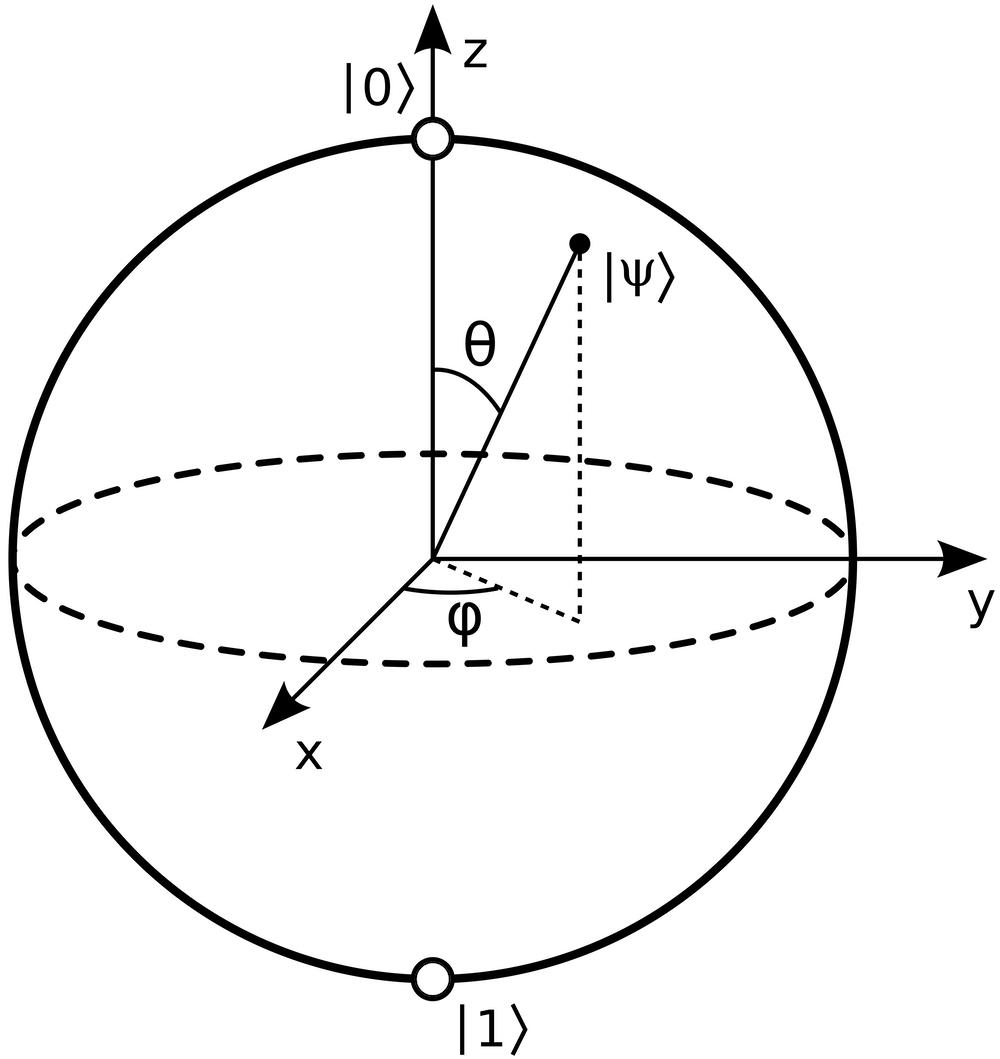
\includegraphics[width=0.5\textwidth]{bloch-sphere.png}
       \caption{Bloch sphere \cite{bloch_sphere}}
    \end{center}
\end{figure} 


In reality, physical qubits can be realized in different ways. There is a plethora of options but the most prominent ones used by leading companies are superconducting qubits and trapped ions (an atom that is not neutral).
\ques{should I also mention that qubits can not be copied? (no-cloning theorem)}
% As opposed to classical bits, qubits have a few more interesting properties that can be worth mentioning.

\subsubsection{Multiple qubits}
Suppose we have two qubits. If these were two classical bits, then there would be four possible states, 00, 01, 10, and 11. Correspondingly, a two-qubit system has four computational basis states denoted $\ket{00}$, $\ket{01}$, $\ket{10}$, $\ket{11}$. A pair of qubits can also exist in superpositions of these four states, so the quantum state of two qubits involves associating a complex coefficient, sometimes called an amplitude, with each computational basis state, such that the state vector describing the two qubits is
$$\ket{\psi} = \alpha \ket{00} + \beta \ket{01} + \gamma \ket{10} + \delta \ket{11}\cite{qc}\text{.}$$

This multiqubit ket notation might be confusing. If we have $\ket{100}$, number $100$ is a binary representation of number $4$. The resulting vector will be eight-dimensional ($2^3 = 8$) with number one at the fourth position (indexing starts from zero). Similarly, $\ket{1111}$ will have number one at the fifteenth position.
\subsection{Measurements}
Measurement is an operation that enables us to find out the state of a qubit, however, this operation does not work as most of us would expect. When we measure a qubit we get either the result 0, with probability $\lvert \alpha \rvert^2$, or the result 1, with probability $\lvert \beta \rvert^2$ \cite{qc}. Naturally, $\lvert \alpha \rvert^2 + \lvert \alpha \rvert^2 = 1$, since the probabilities must sum to one \cite{qc}. Measurement is a destructive operation, upon first measurement, the state of a qubit is collapsed to either $\ket{0}$ or $\ket{1}$, and any subsequent measurements will yield the same result. We can not recover the original state of a qubit after measurement. There are three types of measurements, with respect to axes:
\begin{table}[H]
  \centering
  \begin{tabular}{|c|c|} 
      \hline
      \multicolumn{1}{|c|}{\textbf{Measurement axes}} & \textbf{States}\\
      \hline
      x-axis & $\ket{+} \text{ or }\ket{-}$ \\ 
      \hline
      y-axis & $\ket{-i} \text{ and }\ket{+i}$ \\ 
      \hline
      z-axis & $\ket{0} \text{ or }\ket{1}$ \\ 
      \hline
  \end{tabular}
  \caption{Mesaurements and their respective states}
  \label{tab:measurements-states}
\end{table}
Most (if not all) contemporary quantum computers perform measurements on a computational basis (z-axis). We can also realize measurement on other bases by converting them to computational basis using additional rotation:

\begin{table}[H]
  \centering
  \begin{tabular}{|c|c|} 
      \hline
      \multicolumn{1}{|c|}{\textbf{Measurement axes}} & \textbf{Conversion}\\
      \hline
      x-axis & we apply gate $RY(-\pi/2)$ \\ 
      \hline
      y-axis & we apply gate $RX(\pi/2)$ \\ 
      \hline
      z-axis & we do not have to do anything \\ 
      \hline
  \end{tabular}
  \caption{Mesaurements and their conversion to computational basis~\cite{blog}}
  \label{tab:measurements-conversion}
\end{table}
\todo{consider adding the picture that shows the bases}\\

\subsection{Quantum gates}
Up until now, we have been covering the properties of qubits and the question of how to manipulate qubits is still unanswered. In this section, we will take a closer look at basic quantum gates and we will visualize the operations to make it more easy to digest. They are the quantum equivalent of classical logic gates.

In contrast to logic gates in classical computing, quantum gates are represented by matrices. The only property that the matrix must adhere to is unitarity. There are infinitely many unitary matrices, therefore we have infinitely many quantum gates. \cite{qc}

Another specialty of quantum gates or quantum computation in general is that they are reversible. This means that we can from the output of the gate, we can always determine the input. This is not the case for logic gates. For instance, the $AND$ gate is not reversible. From the output, we cannot determine the input. \cite{qc}

Below are some of the most fundamental gates that are used in quantum computing.
\subsubsection{X gate}
The X gate is a single qubit gate. It is also known as a bit-flip gate because state $\ket{0}$ is flipped to $\ket{1}$ and vice versa \cite{qc}. In simple words, it flips the state by 180 degrees around the x-axis of the block sphere.

\begin{figure}[H]
    \centering
    \begin{minipage}{0.4\linewidth}
      \centering
      $\begin{pmatrix}
        0 & 1 \\
        1 & 0
        \end{pmatrix}$
      \vfill
    \end{minipage}
    \begin{minipage}{0.25\linewidth}
      \centering
      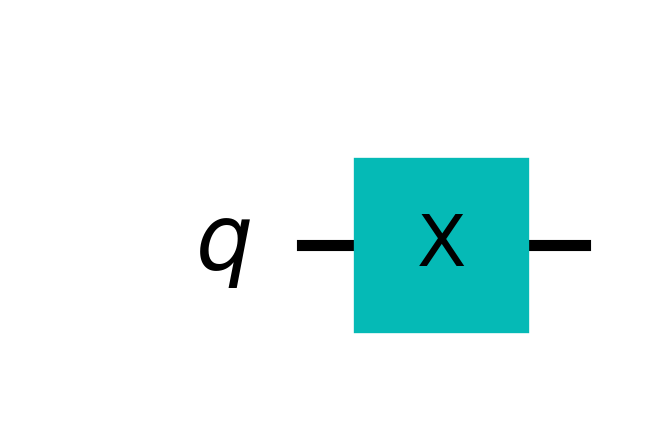
\includegraphics[]{x-gate.png}
      \vfill
    \end{minipage}
    \caption{Matrix and visual representation of the X gate.}
\end{figure}


\qubitRotation{qubit-zero-state.png}{qubit-x-gate.png}{X gate acting on initial state}
\subsubsection{Y gate}
The Y gate flips the state by 180 degrees around the y-axis of the Bloch sphere.
\begin{figure}[H]
    \centering
    \begin{minipage}{0.4\linewidth}
      \centering
      $\begin{pmatrix}
        0 & -i \\
        i & 0
        \end{pmatrix}$
      \vfill
    \end{minipage}
    \begin{minipage}{0.25\linewidth}
      \centering
      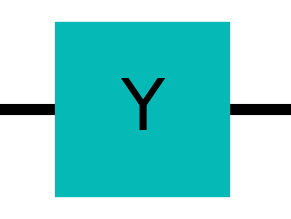
\includegraphics[]{y-gate.png}
      \vfill
    \end{minipage}
    \caption{Matrix and visual representation of the Y gate.}
\end{figure}

\qubitRotation{qubit-zero-state.png}{qubit-y-gate.png}{Y gate acting on initial state}

\subsubsection{Z gate}
This gate also earned a name phase flip. The state $\ket{0}$ leaves intact, but it changes the state $\ket{1}$ to $-\ket{1}$ \cite{qc}. It is a rotation of the state by 180 degrees around the z-axis of the Bloch sphere.
\begin{figure}[H]
    \centering
    \begin{minipage}{0.4\linewidth}
      \centering
      $\begin{pmatrix}
        1 & 0 \\
        0 & -1
        \end{pmatrix}$
      \vfill
    \end{minipage}
    \begin{minipage}{0.25\linewidth}
      \centering
      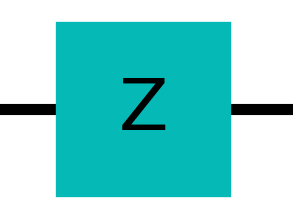
\includegraphics[]{z-gate.png}
      \vfill
    \end{minipage}
    \caption{Matrix and visual representation of the Z gate.}
\end{figure}

\qubitRotation{qubit-superposition.png}{qubit-z-gate.png}{Z gate acting on superposition state}
Note that this time we used a different initial state. If we had started from the initial state, we would have not seen any change.

\subsubsection{Hadamard gate}
The Hadamard operation is just a rotation of the sphere about the y-axis by $\pi/2$, followed by a rotation about the x-axis by $\pi$ \cite{qc}. If we apply Hadamard gate on a qubit in state $\ket{0}$, we get a qubit in an equal superposition of $\ket{0}$ and $\ket{1}$.
\begin{figure}[H]
    \centering
    \begin{minipage}{0.4\linewidth}
      \centering
      $\begin{pmatrix} 
        \frac{1}{\sqrt{2}} &  \frac{1}{\sqrt{2}}  \\
        \frac{1}{\sqrt{2}}  &  -\frac{1}{\sqrt{2}} 
        \end{pmatrix}$
      \vfill
    \end{minipage}
    \begin{minipage}{0.25\linewidth}
      \centering
      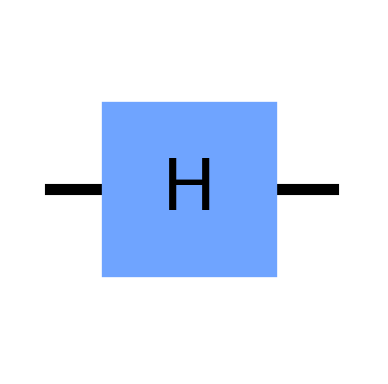
\includegraphics[]{hadamard-gate.png}
      \vfill
    \end{minipage}
    \caption{Matrix and visual representation of the Hadamard gate.}
\end{figure}
\todo{create Hadamard gate state transition visualization}

\subsubsection{Controlled-NOT gate} 
Controlled-NOT (CNOT) gate has two input qubits, known as the control qubit and the target qubit, respectively. The action of the gate may be described as follows. If the control qubit is set to 0, then the target qubit is left alone. If the control qubit is set to 1, then the target qubit is flipped. \cite{qc}

\begin{figure}[H]
  \centering
  \begin{minipage}{0.4\linewidth}
    \centering
    $$\begin{pmatrix}
      1 & 0 & 0 & 0 \\
      0 & 1 & 0 & 0 \\
      0 & 0 & 0 & 1 \\
      0 & 0 & 1 & 0
  \end{pmatrix}$$
    \vfill
  \end{minipage}
  \begin{minipage}{0.25\linewidth}
    \centering
    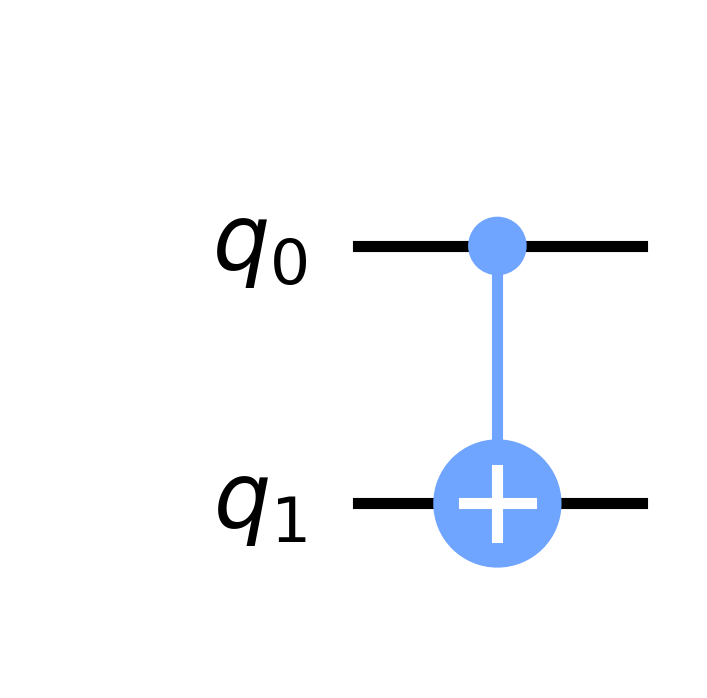
\includegraphics[]{cnot-gate.png}
    \vfill
  \end{minipage}
  \caption{Matrix and visual representation of the CNOT gate.}
\end{figure}

\todo{fix alignment of matrices and gate icon}\\
\todo{consider improving the layout of all the figures, they occupy too much space, maybe I can add a 3x3 table for X, Y, and Z gates that shows qubit state transition, matrix, and gate notation}
\subsection{Quantum entanglement}
Apart from superposition, quantum entanglement is another quantum phenomenon that gives us an advantage over classical computers. When qubits are entangled we mean that they are somehow bound together and they are dependent. Altering the state of one qubit will immediately alter the state of the other qubit in a predictable way. In the below example, we will demonstrate the most simple entangled state, also known as the Bell state.

\begin{figure}[H]
\begin{minipage}{.35\textwidth}
    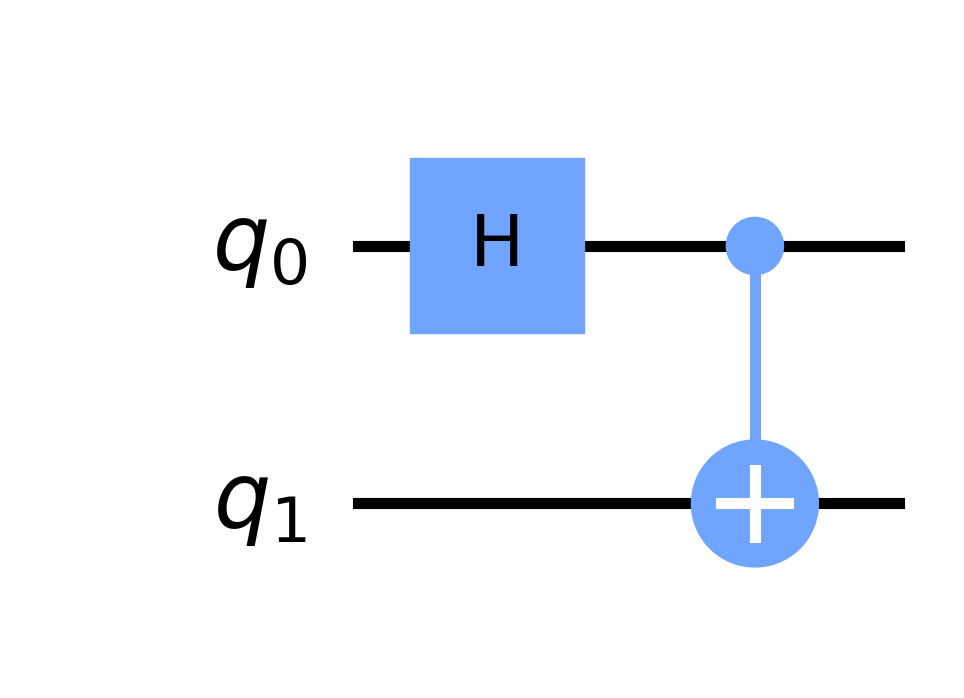
\includegraphics[]{entanglement-circuit.png}
    \caption{Bell state circuit}

\end{minipage}
\hfill
\begin{minipage}{.50\textwidth}
  \begin{align} 
             &\ket{00} = \ket{0} \otimes \ket{0} \label{eq1} \\
             &\frac{1}{\sqrt{2}}(\ket{0} + \ket{1}) \otimes \ket{0} \label{eq2}\\
             &\frac{1}{\sqrt{2}}(\ket{0} \otimes \ket{0} + \ket{1} \otimes \ket{0}) \label{eq3} \\
             &\frac{1}{\sqrt{2}}(\ket{0} \otimes \ket{0} + \ket{1} \otimes \ket{1}) \label{eq4}\\
             &\frac{1}{\sqrt{2}}(\ket{00} + \ket{11}) \label{eq5}
  \end{align}
\end{minipage}
\end{figure}

\noindent In the following lines, we explain individual steps of the computation.\\
\noindent (\ref{eq1}) Initial state of the circuit.\\
(\ref{eq2}) Hadamard gate applied, the first qubit is equally likely to be in state $\ket{0}$ or $\ket{1}$.\\
(\ref{eq3}) Expanded bracket.\\
(\ref{eq4}) CNOT gate applied, it first qubit is $\ket{1}$, state of the second qubit will be flipped\\
(\ref{eq5}) Final state of the circuit.\\

\noindent From the above example, we can see that the qubits are correlated. This particular state is a superposition of only two states $\ket{00}$ and $\ket{11}$, without entanglement we would have to consider a superposition of four states $\ket{00}$, $\ket{01}$, $\ket{10}$, and $\ket{11}$. If the first qubit is measured to be in state $\ket{0}$, then the second one will also be in state $\ket{0}$. The same applies to state $\ket{1}$.

\subsection{Example of quantum computation}
In this section, we will show simple examples to better understand how all the vectors, matrices, and operations work together.

\begin{figure}[H]
    \begin{center}
       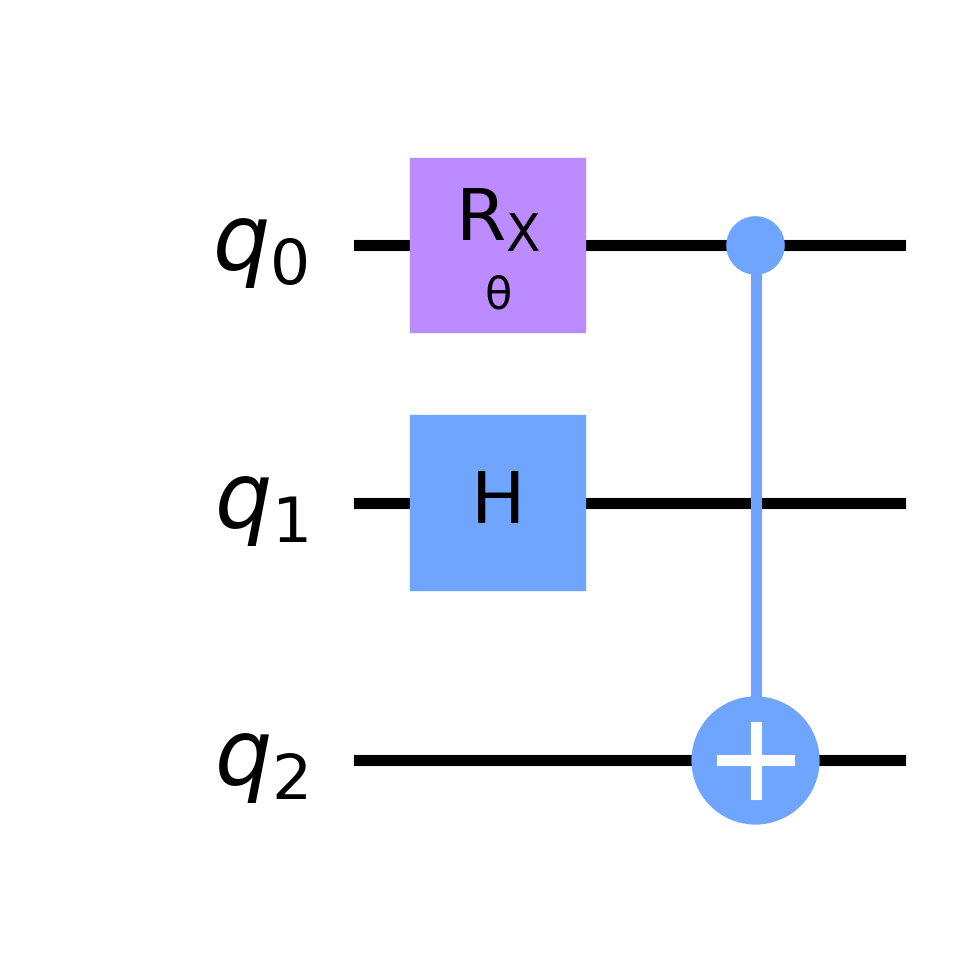
\includegraphics[width=0.5\textwidth]{example-circuit.png}
       \caption{Example circuit}
    \end{center}
\end{figure}

We can proceed in so-called ''columns'' or ''levels''.
At the first level, there is a parametrized RX gate, Hadamard gate, and the third qubit does not have any gate, we can consider that as an identity gate.
$$L_1 = RX \otimes H \otimes I = \begin{pmatrix} 
\cos{\frac{\theta}{2}} & -i\sin{\frac{\theta}{2}} \\
-i\sin{\frac{\theta}{2}} & \cos{\frac{\theta}{2}}
\end{pmatrix} \otimes \begin{pmatrix} 
\frac{1}{\sqrt{2}} &  \frac{1}{\sqrt{2}}  \\
\frac{1}{\sqrt{2}}  &  -\frac{1}{\sqrt{2}} 
\end{pmatrix} \otimes \begin{pmatrix} 
1 & 0 \\
0 & 1
\end{pmatrix}$$
The second level contains a CNOT gate, that acts on the first and third qubit. We will interpret the operation on the second qubit as identity. 
$$ L_2 = CNOT \otimes I = \begin{pmatrix}
1 & 0 & 0 & 0 \\
0 & 1 & 0 & 0 \\
0 & 0 & 0 & 1 \\
0 & 0 & 1 & 0
\end{pmatrix}\otimes\begin{pmatrix} 
1 & 0 \\
0 & 1
\end{pmatrix}$$
Our circuit consists of three qubits. Every qubit is initialized in a state $\ket{0}$, we have three of them, therefore our initial state is $\ket{000}$. To obtain the final matrix of the circuit we need to multiply the initial state with matrices $L_1$ and $L_2$.
$$RESULT = \ket{000}L_{1}L_2$$
Notice that, if we would not have used identity gates, eventually we would run into a problem with matrix dimensions incompatibility when doing matrix multiplication.

\subsection{Noisy Intermediate-Scale Quantum (NISQ) computers}
In today's world, quantum computers still suffer from several problems, namely the following ones.

\subsubsection{Scalability}
The more qubits we have, the bigger instances of problems we can solve. However, with an increasing number of qubits, and the number of gates we introduce errors into quantum computation. The gates themselves, especially the entangling ones, possess a certain probability that the outcome of the gate will result in an error. Also, qubit connectivity goes hand in hand with the scalability. It does not make sense to have a large number of qubits if they are not connected and we can not use multiqubit gates on them.

\subsubsection{Quantum decoherence}
Qubits are very sensitive and their state can be easily influenced by the noise from the environment. By noise we mean magnetic fields, radio waves, vibrations, light, and more. To minimize this effect, quantum processing units (QPUs) are accompanied by other components that are used to shield the qubits from the environment and keep them at temperatures close to absolute zero ($0$K = $-273.15^{\circ}$C). Thanks to that quantum computers are large in size and they often resemble chandeliers even though QPUs are in size comparable to processors in personal standard computers.

\subsubsection{Lack of error correction}
Theoretically, we always consider so-called logical qubits that do not have any problems and work seamlessly. In reality, we use physical qubits that suffer from noise and decoherence and it hinders us from executing quantum algorithms reliably. To mitigate this problem, we can use quantum error correction. The idea is that we can use multiple physical qubits, from tens even to thousands, to create a single reliable logical qubit. But doing so we run into a problem with scalability. 

\paragraph{}
Quantum computers that match these characteristics are called noisy intermediate-scale quantum (NISQ) computers. Here ''intermediate scale'' refers to the size of quantum computers that will be available in the next few years, with a number of qubits ranging from 50 to a few hundred. ''Noisy'' emphasizes that we'll have imperfect control over those qubits. The noise will place serious limitations on what quantum devices can achieve in the near term \cite{preskill_nisq}.


\section{Ground state energy}
Before getting into ground state energy let's revisit an atom first. Atoms are the basic building blocks of matter. They are the smallest units of an element that can combine with other elements. Atoms are composed of 3 subatomic particles, protons, neutrons, and electrons. Protons and neutrons reside in the tiny nucleus of the atom. As their names suggest, protons have a positive electrical charge, while neutrons are electrically neutral. The vast majority of an atom's volume is the space in which the electrons reside. Electrons have a negative electrical charge. The electrons are attracted to the protons in the nucleus by the electrostatic force that exists between particles of opposite electrical charge. Every atom has an equal number of electrons and protons, so atoms have no net electrical charge.

Electrons are grouped into orbitals. Each orbital has a characteristic shape and energy. An electron can ''jump'' from one allowed orbit to another by either absorbing or emitting photons whose energy corresponds exactly to the energy difference between the two orbits. The electron must absorb energy in order to move to a higher-energy state. Conversely, energy is emitted when the electron jumps to a lower-energy state. The lowest-energy state is called the ground state of the atom. When the electron is in a higher-energy state the atom is said to be in an excited state \cite{chemistry}. We will measure this energy in a hartree (Ha) units. Hartree is a unit of energy in the atomic units system.~\cite{hartree}
\todo{picture of transition from the ground state to excited state and then back to the ground state}
\todo{picture of energy levels}

\section{Hamiltonian}
Hamiltonian defines the total energy of a physical system. Many different forms of Hamiltonians exist in physics and chemistry, but we will not go into details. For us is important that once a Hamiltonian is constructed, it must be translated into operators that can be directly measured on a quantum computer. The representation for quantum computer looks as follows:
$$\hat{H} = \sum_{i=1}^{m}c_i\sigma_i \text{, } \sigma_i \in \{I, X, Y, Z\}^{\otimes n}\text{, } c_i \in \mathbb{R} \text{, }$$ 
where $I$ is an identity matrix and $X$, $Y$, $Z$ are Pauli matrices which we discussed in the section \ref{sec:pauli-matrices}.~\cite{fedorov2021vqe}

The Pauli matrices represent measurements. This expression, $c_{1}Z_{0}X_{1}Y_{2}$, means that we measure qubit zero on the z-axis, qubit one on the x-axis, and qubit two on the y-axis and we will multiply the results together with the coefficient $c_{1}$. Sometimes this Hamiltonian representation is referred to as a sum of Pauli strings. The specialty of this representation of Hamiltonian is that it forms a Hermitian matrix and Hermitian matrices have real eigenvalues.